\documentclass[10pt]{beamer}

%packages
\usepackage[english]{babel}
\usepackage[utf8]{inputenc}
\usepackage{graphicx}

%themes
\usetheme{Dresden}
\usecolortheme{rose}
\useoutertheme{tree}
\setbeamertemplate{caption}[numbered]

%general
\title{Poor harvest in India in 2002 shown with CDC wheather data}
\author{Tilman Hinnerichs, Anja Reusch, Veronika Soloviova}
\institute{Bertelsmann Data Science Scholarship Program}
\date{\today}

\begin{document}
\begin{frame}
	\titlepage
\end{frame}

\begin{frame}{What question would we like to answer?}
	On the search for good data we stumbled accross the CDC (Climate Data Center) of the DWD (German Wheather Center). They are providing data from all kinds of different wheather stations all around the world as we visualized in Figure~\ref{Stations}.
	\begin{figure}[ht]
		\centering
		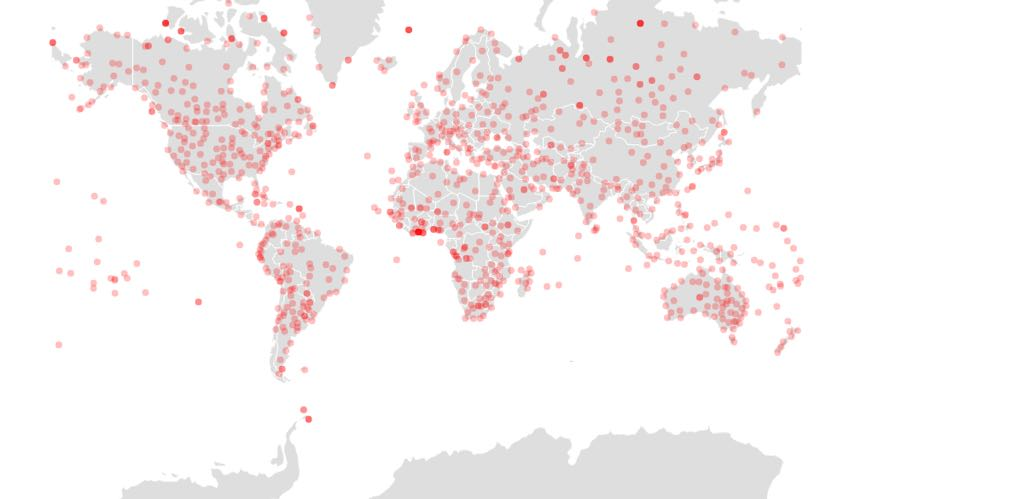
\includegraphics[width = 0.5\textwidth]{WheatherStations.jpeg}
		\caption{Wheather stations provided by the CDC}
		\label{Stations}
	\end{figure}
\end{frame}	

\begin{frame}{What question would we like to answer?}
	The CDC is providing all different kinds of data for those stations. Their database holds the statistics on snowfall, precipitation and sunshine hours and literally everything. The data is provided in a raw heap of data which we tried to classify.\\\vfill
	\large But what to do with that giant pile of data?
\end{frame}

\begin{frame}
	Hence, we found another source of data: The \textbf{Food and Agriculture Oranization of the United Nation}, which provides data on quantitative measurements of the yield of harvest. There we found a peak in the yield of paddled Rice of India in 2002, seen in Figure~\ref{IndiaRice}, where more than 22\% of the production got lost.
	\begin{figure}
		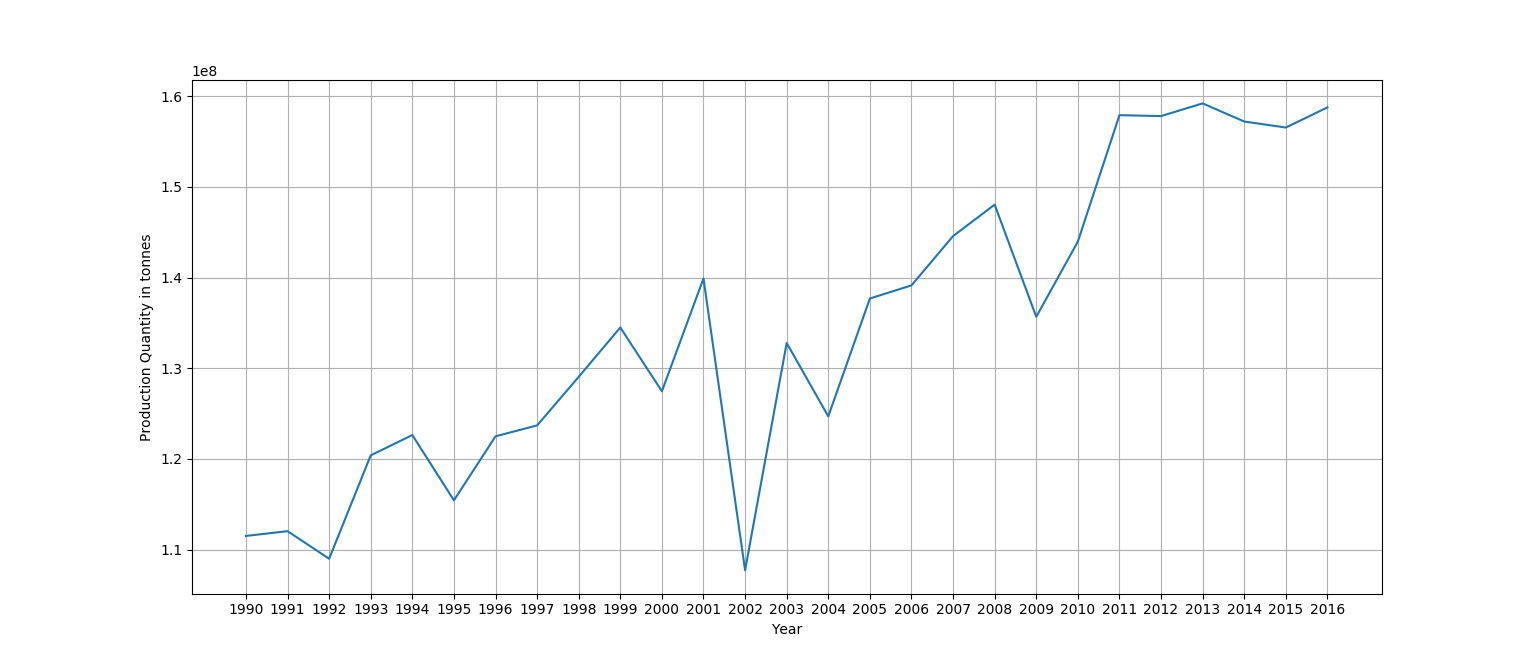
\includegraphics[width=1\textwidth]{IndiaRiceQuantity.png}
		\caption{We can see a harsh peek at 2002}
		\label{IndiaRice}
	\end{figure}
\end{frame}

\begin{frame}{What question would we like to answer?}
	So we would like to know: \\
	\begin{itemize}
		\item \large Can we see possible reasons for this peak in our wheather data?
	\end{itemize}
\end{frame}

\begin{frame}
	We therefor had a look at the rice production on the world shown below in Figure~\ref{RiceYield}. Even though it is showing the productivity, it is nevertheless a good indicator for the absolute production.
	\begin{figure}
		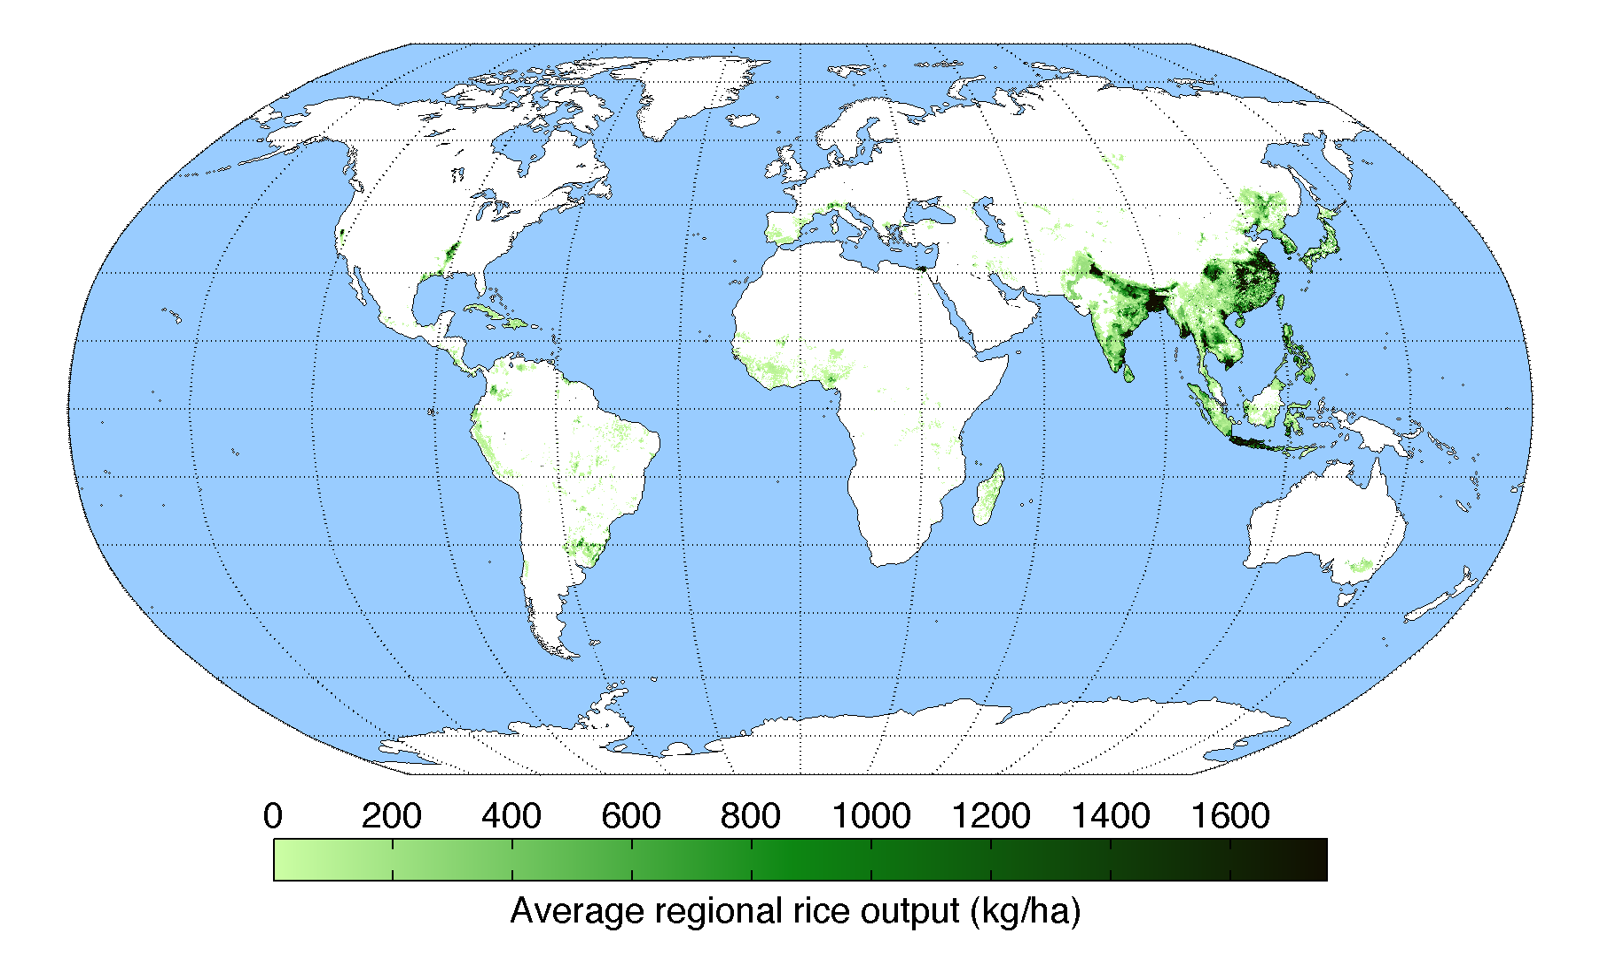
\includegraphics[width=0.75\textwidth]{RiceYield.png}
		\label{RiceYield}
		\caption{World rice production highlighted}
	\end{figure}
\end{frame}

\begin{frame}
	So first have a look at the common rice crops in India and their growth and harvest time intervals. Here we can see the Kharif and the Rabi crop displayed for India.
	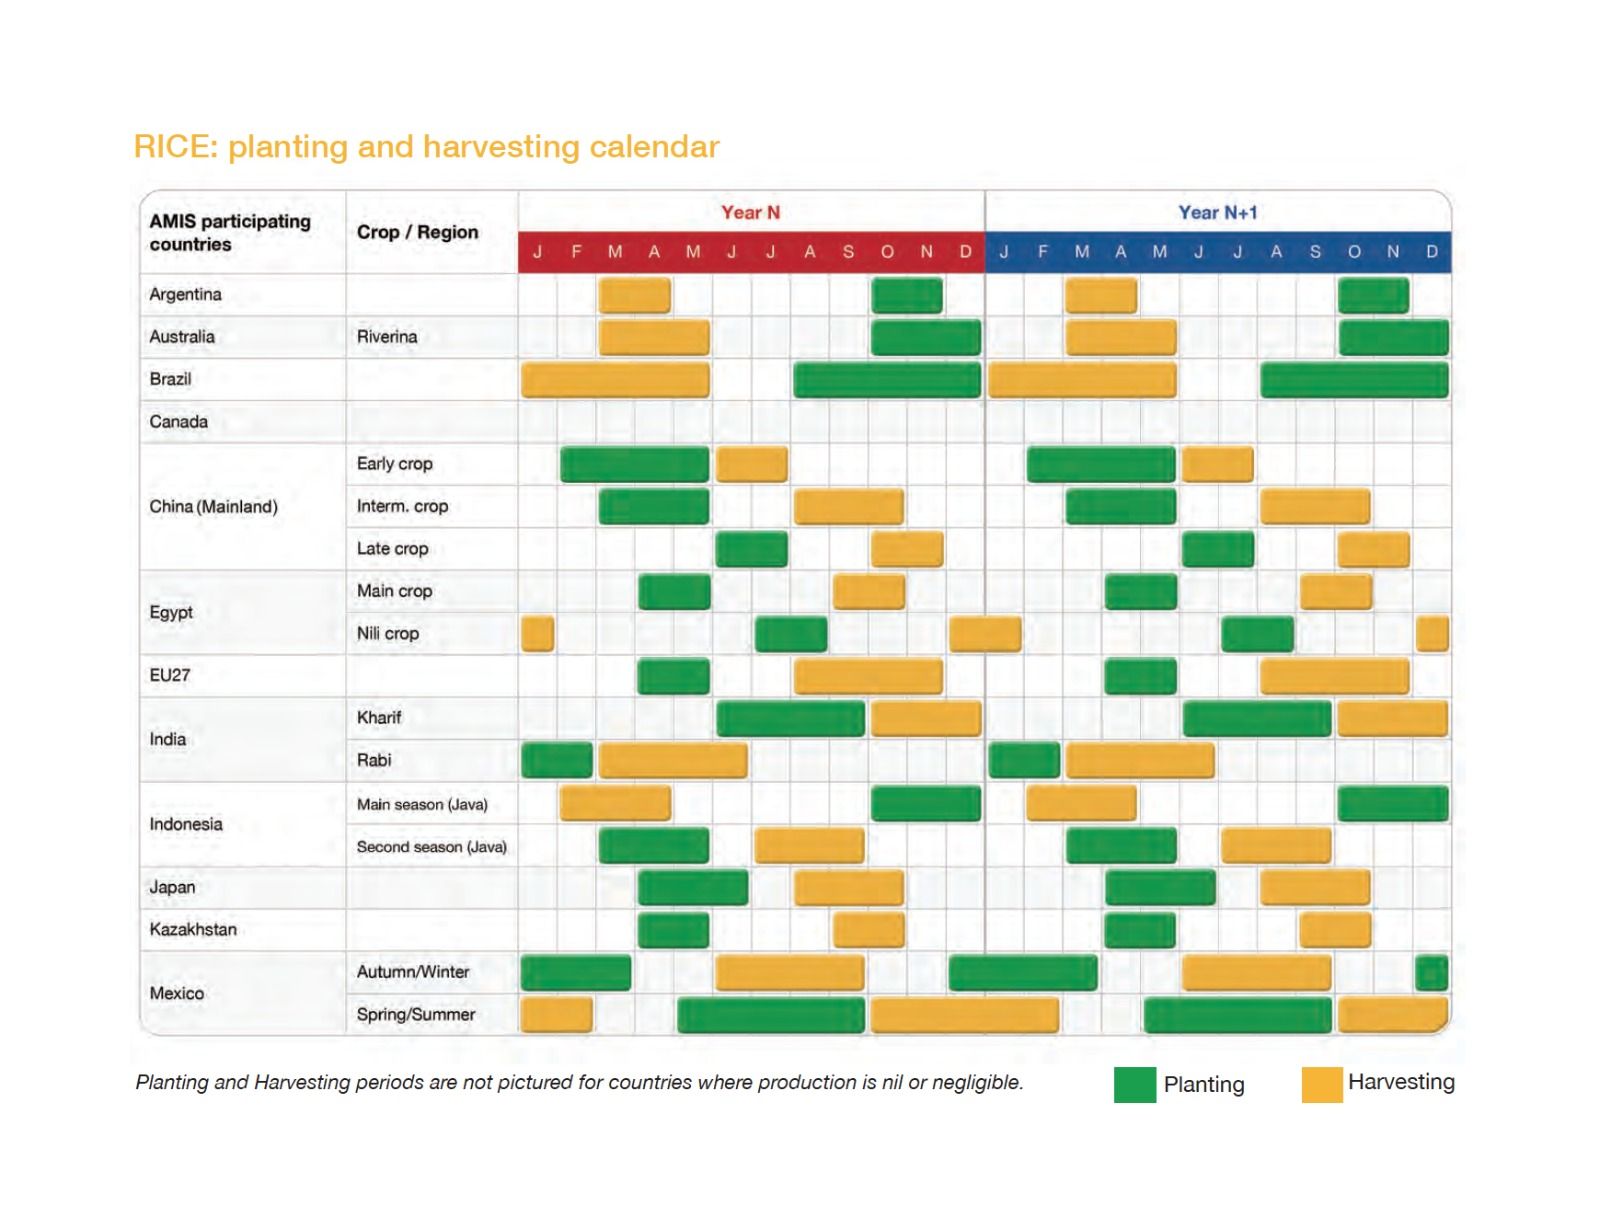
\includegraphics[width=1\textwidth]{RiceCrops.jpeg}
\end{frame}

\begin{frame}
	Now lets have a look at our wheather data for some city located in the productice are of India concerning rice cultivation. \\
	We therefore considered the following cities, while rejecting cities not including the crucial data:
	\begin{itemize}
		\item Guwahati,
		\item Cherrapunji,
		\item Daltonganj,
		\item Jagdalpur,
		\item Chennai Minambakkam, and
		\item Bangalore
	\end{itemize}
\end{frame}

\begin{frame}
	Now concerning the crucial diagrams (You can get the data and the other diagrams on request):
	\begin{columns}
		\begin{column}{0.5\textwidth}
			\begin{figure}
				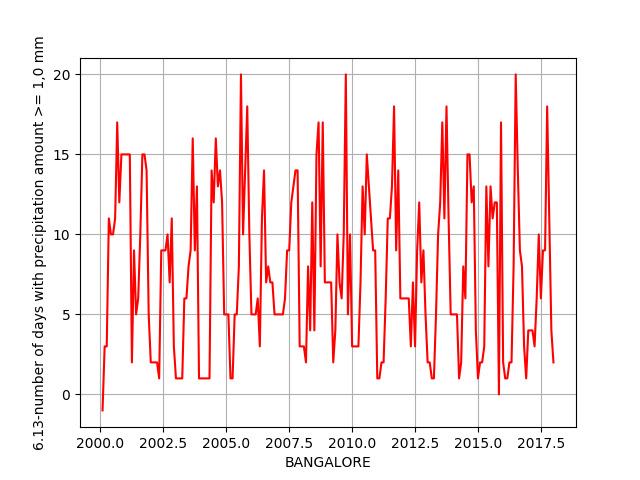
\includegraphics[width=1.2\textwidth]{BangalorePrecipitation1mm.png}
				\caption{Precipitation for Bangalore}
			\end{figure}
		\end{column}
		\begin{column}{0.5\textwidth}
			\begin{figure}
				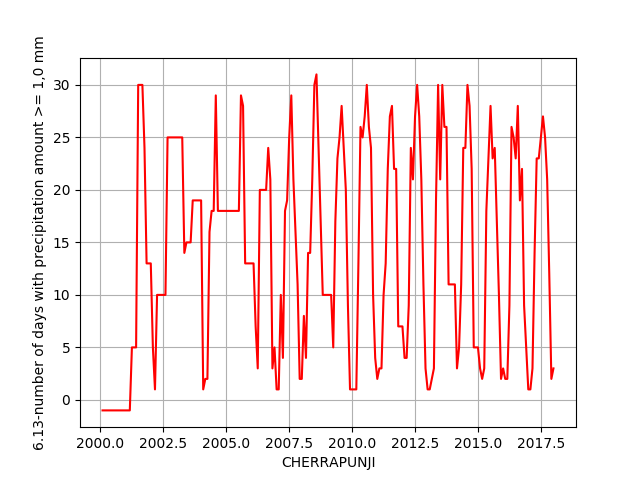
\includegraphics[width=1.2\textwidth]{CherrapunjiNumberOfDays1mm.png}
				\caption{Precipitation for Cherrapunji}
			\end{figure}
		\end{column}
		
	\end{columns}
	Considering those we can see the cut in the middle of year 2002.
\end{frame}

\begin{frame}
	\begin{itemize}
		\item \large Hence, we can see a that the Kharif Crop, which is decisive for the production quantity, had to suffer a lot under the wheather conditions given in 2002
	\end{itemize}
	
\end{frame}

\begin{frame}{Sources}
	\begin{itemize}
		\item This presentation was build using the data of the previously mentioned sites
		\item Plots and analysing has been done with several python libraries, e.g. Matplotlib, Pandas, NumPy, etc., and Vega
	\end{itemize}
	Other sources:\\
	\vspace{0.25cm}
	\begin{tabular}{rl}
		RICE: planting and harvesting calendar:& AMIS Crop Calendar\\
		Figure 3:&Wikipedia
	\end{tabular}
\end{frame}

\end{document}